\chapter{Draft: Level Set XFEM Topology Optimization of 3D Navier-Stokes and Scalar Transport Problems}
\label{sec:level_set_XFEM_topology_optimization_of_3D_navier_stokes_and_scalar_transport_problems}

% \documentclass[twocolumn]{svjour3}

% \smartqed

% \usepackage{fix-cm}
% \usepackage{graphicx}
% \usepackage{fixltx2e}
% \usepackage{dblfloatfix}
% \usepackage{subfig}
% \usepackage{tabularx}
% \usepackage{natbib}                        % Use citep, citet in citations
% \usepackage{amsmath,mathtools}             % Cases
% \usepackage{color}                         % Color text to indicate changes
% \usepackage{multirow}                      % More complex tables
% \usepackage{chngcntr}                      % Show section in table

% \counterwithout{table}{section}

% \journalname{Computational Mechanics}

% \begin{document}

% -----------------------------------------------------------------------------
% Title

% \title{Density and Level Set-XFEM Schemes for Topology Optimization of 3-D Structures}

% \subtitle{Topology Optimization in 3D}

% \author{Carlos H. Villanueva	\and Kurt Maute}

% \institute{
% 	C. H. Villanueva \at
% 	Department of Mechanical Engineering,\\
% 	University of Colorado at Boulder,\\
% 	Boulder, CO 427 UCB, USA\\
% 	e-mail: carlos.villanueva@colorado.edu\\
% 	\and
%	K. Maute \at
% 	Department of Aerospace Engineering,\\
% 	University of Colorado at Boulder,\\
% 	Boulder, CO 427 UCB, USA\\
% 	e-mail: maute@colorado.edu\\
% 	}

% \date{Received: date / Accepted: date}

% \maketitle

% -----------------------------------------------------------------------------
% Abstract

% \begin{abstract}

This paper studies level set topology optimization of incompressible Stokes and Navier-Stokes flow, and scalar transport problems in three-dimensions. The paper expands on previous work on the LSM-XFEM by \citep{MM:14,VM:14} to three-dimensional fluid and scalar transport problems. The focus of the study is to analyze the correct application of boundary conditions at the level set interface to be able to model high Reynolds number flow in optimization problems. Accurate enforcement of boundary conditions will be done through the Nitsche method \citep{BH:12}, and the ghost penalty formulation \citep{SRG+:14}. Using these approaches, we will generate a robust optimization approach capable of handling multiple discontinuities at the cut elements, and modeling coupled physics such as fluid flow and advection-diffusion problems.

As the level set method can accurately describe the discontinuities in the design domain, and the capabilities of additive manufacturing techniques increase, our work will study a curvature regularization technique to increase the smoothness of the level set interface in order to create better-looking designs.
Our work illustrates that the LSM-XFEM optimization approach is an ideal tool to generate optimized geometries that can be easily manufactured using the capabilities of three-dimensional printing.

% \keywords{eXtended Finite Element Method \and Topology Optimization \and
% Solid Isotropic Material with Penalization \and Level Set Methods \and Additive Manufacturing \and 3D Printing}
% 
% \end{abstract}

% -----------------------------------------------------------------------------
% Introduction

\section{Methodology}
\label{sec:fluids_methodology}

We consider an incompressible Navier-Stokes problem in a two-phase domain with $\Omega = \Omega^{+} \cup \Omega^{-}$, where $\Omega^{k}$ denotes the domain occupied by phase $k \in \lbrace +, - \rbrace$. The interface between the phases is denoted by $\Gamma_{\mathrm{int}} = \Omega^{+} \cap \Omega^{-}$. The domain $\Omega$ is governed by the incompressible Navier-Stokes equations, which are given in convective form as
%
\begin{equation}
	\centering
	\label{eq:incompressible_Navier_Stokes}
	\rho^{k} \frac{\partial \mathbf{u}^{k}}{\partial t}	+ 
	\rho^{k} \mathbf{u}^{k} \cdot \nabla \mathbf{u}^{k} +
	\nabla p^{k} - 2\mu^{k} \nabla \cdot \boldsymbol{\varepsilon} \left( \mathbf{u}^{k} \right) = \rho^{k} \mathbf{g} \quad \text{in $\Omega^{k}$}
\end{equation}
%
\begin{equation}
	\centering
	\label{fig:incompressibility}
	\nabla \cdot \mathbf{u}^{k} = 0 \quad \text{in $\Omega^{k}$}
\end{equation}
%
\noindent
where $\rho^{k}$ and $\mu^{k}$ represent the density and the dynamic viscosity of the fluid for phase $k$.  $\mathbf{u}^{k}$ is the velocity and $p^{k}$ is the pressure in the phase $k$. $\boldsymbol{\varepsilon} = \frac{1}{2} \left( \nabla \mathbf{u}^k + \left( \nabla \mathbf{u}^k \right)^{T} \right)$ is the rate-of-deformation tensor. $\mathbf{g}$ is the gravity vector.

Initial conditions are applied in $\Omega^{k}$, and boundary conditions on the outer part of $\Gamma^{k}$, where $\Gamma^{k}$ represents the boundary of the domain $\Omega$.

At time $t=0$, a divergence-free velocity field is defined as
%
\begin{equation}
	\centering
	\label{eq:initial_conditions}
	\mathbf{u}^{k}\left( \mathbf{x}, t=0 \right) = \mathbf{u}^{k}_{0}\left( \mathbf{x} \right) \quad \text{$\Omega^{k}$}
\end{equation}
%
Dirichlet and Neumann boundary conditions are applied on $\Gamma_{D}^{k}$ and $\Gamma_{N}^{k}$ as
%
\begin{equation}
	\centering
	\label{eq:dirichlet_boundary_conditions}
	\mathbf{u}^{k} = \mathbf{u}^{k}_{D} \quad \text{on $\Gamma^{k}_{D}$}
\end{equation}
%
\begin{equation}
	\centering
	\label{eq:neumann_boundary_conditions}
	\boldsymbol{\sigma}\left(\mathbf{u}^{k},p^{k}\right) \cdot \mathbf{n}^{k} = \mathbf{h}^{k} \quad \text{on $\Gamma^{k}_{N}$}
\end{equation}
%
\noindent
where $\boldsymbol{\sigma}\left(\mathbf{u}^{k},p^{k}\right) = -p^{k}\mathbf{I} + 2\mu^{k}\boldsymbol{\varepsilon} \left( \mathbf{u}^{k} \right)$ represents the Cauchy stress tensor. The boundary of the subdomain $\Omega^{k}$ is represented with $\Gamma^{k} = \Gamma^{k}_{D} \cup \Gamma^{k}_{N} \cup \Gamma_{\mathrm{int}}$.

Additional interface conditions must be used to enforce continuity of the solution at the interface of the subdomains:
%
\begin{equation}
	\centering
	\label{eq:solution_continuity}
	[\mathbf{u}] = 0 \quad \text{on $\Gamma_{\mathrm{int}}$}
\end{equation}
%
\noindent
where $[\cdot]$ represents the jump operator across a phase boundary as
%
\begin{equation}
	\centering
	\label{eq:velocity_continuity}
	[\mathbf{u}] = \mathbf{u}^{+} - \mathbf{u}^{-}
\end{equation}
%
Surface tension effects are balanced by a jump in the traction:
%
\begin{equation}
	\centering
	\label{eq:stress_continuity}
	[\boldsymbol{\sigma}(\mathbf{u},p) \cdot \mathbf{n}_{\mathrm{int}}] = -\gamma \kappa \mathbf{n}_{\mathrm{int}} \quad \text{on $\Gamma_{\mathrm{int}}$}
\end{equation}
%
\noindent
where $\gamma$ is the surface tension coefficient, and $\kappa = \nabla \cdot \mathbf{n}_{\mathrm{int}}$ is the curvature of the phase boundary.

A Streamline Upwind Petrov/Galerkin (SUPG) \citep{TMR+:92} and a Pressure Stabilizing Petrov/Galerkin (PSPG) \citep{BH:82} schemes are used to alleviate numerical instabilities and resolve the subgrid-scale components.

Assuming discrete trial functions spaces $\mathbf{u}^{k}_{h} \in V_{\mathbf{u},h}^{k}$ for the velocity, and $p^{k}_{h} \in V_{p,h}^{k}$ for the pressure, as well test functions $\mathbf{v}^{k}_{h} \in \hat{V}_{\mathbf{v},h}^{k}$ for the velocity, and $q^{k}_{h} \in \hat{V}_{p,h}^{k}$ for the pressure, we seek $\left(\mathbf{u}^{k}_{h}, p^{k}_{h}\right) \in V^{k}_{\mathbf{u},h} \times V_{p,h}^{k}$ such that
%
\begin{multline}
	\label{eq:incompressible_Navier_Stokes_stabilization}
	\int \mathbf{v}^{k}_{h} \rho^{k} \frac{\partial \mathbf{u}^{k}_h}{\partial t} \, \mathrm{d}\Omega^{k} + 
	\int \mathbf{v}^{k}_{h} \rho^{k} \mathbf{u}^{k}_{h} \cdot \nabla \mathbf{u}^{k}_{h} \, \mathrm{d}\Omega^{k} - 
	\int \nabla \cdot \mathbf{v}^{k}_{h} p^{k}_{h} +  \, \mathrm{d}\Omega^{k} + 
	\int 2 \boldsymbol{\varepsilon} \left( \mathbf{v}^{k}_{h} \right) \mu^{k} \boldsymbol {\varepsilon} \left( \mathbf{u}^{k}_{h} \right) \, \mathrm{d}\Omega^{k} + \\
	\int \rho^{k} \mathbf{u}^{k}_{h} \cdot \nabla \mathbf{v}^{k}_{h} \tau^{k}_{M} \mathbf{r}^{k}_{M,h} \, \mathrm{d}\Omega^{k} + \int \nabla \cdot \mathbf{v}^{k}_{u} \tau^{k}_{C} \mathbf{r}^{k}_{C,h} \, \mathrm{d}\Omega^{k} + 
	\int \nabla q^{k}_{h} \tau^{k}_{M} \mathbf{r}^{k}_{M,h} \, \mathrm{d}\Omega^{k} - \\
	\int q^{k}_{h} \nabla \cdot \mathbf{u}^{k}_{h} \, \mathrm{d}\Omega^{k} + \int \mathbf{v}^{k}_{h} \boldsymbol{\sigma}\left( \mathbf{u}^{k}_{h}, p^{k}_{h} \right) \cdot \mathbf{n}^{k} \, \mathrm{d}\Gamma_{\mathrm{int}} = \int \mathbf{v}^{k}_{h} \rho^{k} \mathbf{g} \, \mathrm{d}\Omega^{k} + \int \mathbf{v}^{k}_{h} \mathbf{h}^{k} \, \mathrm{d}\Gamma^{k}_{N}
\end{multline}
%
\noindent
where $\mathbf{r}^{k}_{M,h}$ is the discrete residual of the momentum equation:
%
\begin{equation}
	\centering
	\label{eq:discrete_residual_momentum}
	\mathbf{r}^{k}_{M,h} = \rho^{k} \frac{\partial \mathbf{u}^{k}_h}{\partial t} + \rho^{k} \mathbf{u}^{k}_{h} \cdot \nabla \mathbf{u}^{k}_{h} + \nabla p^{k}_{h} - 2\mu^{k} \nabla \cdot \boldsymbol{\varepsilon}\left( \mathbf{u}^{k}_{h} \right) - \rho^{k} \mathbf{g}
\end{equation}
%
\noindent
and $\mathbf{r}^{k}_{C,h}$ is the discrete residual of the continuity equation:
%
\begin{equation}
	\centering
	\label{eq:discrete_residual_continuity}
	\mathbf{r}^{k}_{C,h} = \nabla \cdot \mathbf{u}^{k}_{h}
\end{equation}
%
\noindent
$\tau^{k}_{M}$ and $\tau^{k}_{C}$ represent the SUPG and PSPG stabilization parameters, respectively.

We apply Nitsche's method \citep{Nitsche:75, Hansbo:05} for the weak imposition of the velocity continuity described in Equation \ref{eq:velocity_continuity}, and face-oriented ghost-penalty stabilization terms for each subdomain in the interface zone \citep{BH:12, SW:14}.

Analogous to the structural topology optimization problem of \citep{VM:14}, we introduce fictitious springs to pin free floating material in ``fluid-void'' problems.
%
\begin{equation}
	\centering
	\mathbf{r}^{k}_{P,h} = \mathbf{v}^{k}_{h} k_{p} p^{k}_{h}
\end{equation}
%
where $k_{p}$ denotes the stiffness of the distributed system of springs.

% -----------------------------------------------------------------------------

\section{Numerical examples}
\label{sec:numerical_examples}

We study our LSM-XFEM approach with numerical examples for incompressible Navier-Stokes and scalar transport problems in three dimensions. Four numerical examples will be used: a) a pipe bend, b) a diffuser, c) a micromixer, and d) a fluid duct with heat source.

In all examples, the optimization problems are solved by the Globally Convergent Method of Moving Asymptotes (GCMMA) of \citep{Svanberg:95, Svanberg:02}. The sensitivities are computed by the adjoint method. The design domains are discretized by eight-node linear elements. The linear systems of the forward and adjoint problems are solved by a parallel implementation of the GMRES method \citep{Trilinos:03} The problems are preconditioned by an ILU factorization with a fill of 2.0 and an overlap of 1.0. The convergence tolerances for both, the GCMMA and the GMRES solver, are chosen sufficiently low such that the optimization results do not depend on the tolerance values. The pressure spring stiffness value, $k_{p}$, is $10^{-6}$. Geometric and material parameters are
given in non-dimensional and self-consistent units.

% -----------------------------------------------------------------------------

\subsection{Optimization criteria}
\label{sec:optimization_criteria}

This section details the objective and constraints criteria used in the optimization problems.

The pressure drop criteria measures the difference of the average total pressure between the inlet and the outlet:
%
\begin{equation}
	\centering
	\label{eq:pressure_drop_criteria}
	F_{\mathrm{PD}} =
	\frac{\int p^{f}_h + \frac{\rho^{f} \vert \mathbf{u}^{f}_h \vert^2}{2} \,\mathrm{d}\Gamma_{\mathrm{in}}}{\int \,\mathrm{d}\Gamma_{\mathrm{in}}} -
	\frac{\int p^{f}_h + \frac{\rho^{f} \vert \mathbf{u}^{f}_h \vert^2}{2} \,\mathrm{d}\Gamma_{\mathrm{out}}}{\int \,\mathrm{d}\Gamma_{\mathrm{out}}}
\end{equation}
%
\noindent
where the superscript $f$ represents the value over the fluid phase.

To measure the maximum difference between a current scalar field and a target scalar value, we use the Kreisselmeier-Steinhauser function \citep{KS:79}:
%
\begin{equation}
	\centering
	\label{eq:target_scalar_value_criteria}
	F_{\mathrm{TSV}} =
	\frac{1}{\beta^{f}} \ln \int e^{\beta\left( T^{f}_{h} - T_{\mathrm{ref}}^{f} \right)^2} \,\mathrm{d}\Gamma
\end{equation}
%
where a larger value of $\beta^{f}$ increases the enforcement of the function, but may result in numerical overflow.

The volume of the fluid and void (or solid) phase regions is computed as:
%
\begin{equation}
	\centering
	\label{eq:fluid_volume_criteria}
	F_{\mathrm{volume},f} =
	\int \,\mathrm{d}\Omega^{f}
\end{equation}
%
\begin{equation}
	\centering
	\label{eq:solid_volume_criteria}
	F_{\mathrm{volume},s} =
	\int \,\mathrm{d}\Omega^{s}
\end{equation}
%
The perimeter criteria is computed as:
%
\begin{equation}
	\centering
	\label{eq:perimeter_criteria}
	F_{\mathrm{perimeter}} = \int \,\mathrm{d}\Gamma_{\mathrm{int}}
\end{equation}
%
% -----------------------------------------------------------------------------

\subsection{Pipebend and Diffuser}
\label{sec:pipebend_and_diffuser}

We consider the bend and diffuser ``fluid-void'' problems depicted in Figures \ref{fig:pipebend_setup} and \ref{fig:diffuser_setup}. The problems were adapted to three dimensions from their two dimensional equivalents found in \citep{BP:03,KM:12,MM:14}.
%
\begin{figure}
	\centering
	\includegraphics[width=0.75\linewidth]{pipebend_setup.eps}
	\caption{Setup for the pipebend problem. A parabolic inlet flow in the $x$-direction, with a maximum value of $1.0$ enters the design domain through a circular inclusion of diameter $L$ in the minimum YZ facet. The outlet is modeled as a circle with diameter $L$ and is located in the minimum $XZ$ facet with a constant pressure of $1.0$.}
	\label{fig:pipebend_setup}
\end{figure}
%
\begin{figure}
	\centering
	\includegraphics[width=0.75\linewidth]{diffuser_setup.eps}
	\caption{Setup for the diffuser problem. A parabolic inlet flow in the $x$-direction, with a maximum value of $1.0$ enters the design domain through the entire minimum YZ facet. The outlet, modeled as a circle of diameter $\frac{5}{3}L$ is located in the maximum YZ facet with a constant pressure of $1.0$.}
	\label{fig:diffuser_setup}
\end{figure}
%
This example seeks to study the capability of our LSM-XFEM approach to model three-dimensional ``fluid-void''  incompressible Stokes and Navier-Stokes flows, with low and high Reynolds numbers. In contrast to density methods, our framework does not model fluid in the void phase. The design variables are fixed at the inlet and outlet to be in the fluid phase to ensure the correct enforcement of the boundary conditions. A velocity of $1$ in the $x$-direction is prescribed at the inlet, and a pressure of $1$ is prescribed at the outlet. For both, the bend and diffuser problems, we will model a Stokes flow with $Re=1$, a Navier-Stokes flow with $Re=1$, and a Navier-Stokes flow with a $Re=100$. The initial designs for the bend and diffuser are shown in Figures \ref{fig:pipebend_initial_design} and \ref{fig:diffuser_initial_design}. The complete list of parameters for the problem setup are shown in Tables \ref{tab:bend_parameters} and \ref{tab:diffuser_parameters}.
%
\begin{table}
	\centering
	\begin{tabular*}{0.75\textwidth}{l l}
	\hline
	Outlet pressure             & 1.0 \\
	Reynolds number             & 1.0 \\
    Inlet velocity              & $u^{f}_{h_{x}} = 1.0$ \\
    Element length              & $h=0.083333$ \\
    Maximum volume fraction     & $\bar{v}_{f} = 0.25$ \\
    Pressure difference penalty & $w_{\mathrm{pres}} = 1.0$ \\
    Perimeter penalty           & $w_{\mathrm{per}} = 0.01$ \\
	Smoothing filter            & $d = 2.4 \cdot h$ \\
	\hline
	\end{tabular*}
	\caption{Parameters for bend problem.}
	\label{tab:bend_parameters}
\end{table}
%
\begin{table}
	\centering
	\begin{tabular*}{0.75\textwidth}{l l}
	\hline
	Outlet pressure             & 1.0 \\
	Reynolds number             & 1.0 \\
    Inlet velocity              & $u^{f}_{h_{x}} = 1.0$ \\
    Element length              & $h=0.083333$ \\
    Maximum volume fraction     & $\bar{v}_{f} = 0.5$ \\
    Pressure difference penalty & $w_{\mathrm{pres}} = 1.0$ \\
    Perimeter penalty           & $w_{\mathrm{per}} = 0.01$ \\
	Smoothing filter            & $d = 2.4 \cdot h$ \\
	\hline
	\end{tabular*}
	\caption{Parameters for diffuser problem.}
	\label{tab:diffuser_parameters}
\end{table}
%
\begin{figure*}
	\centering
	\begin{tabularx}{\linewidth}{XX}
		\subfloat[Symmetrical clip along the XY facet of the fluid phase.]{
			\label{fig:pipebend_initial_design_fluid}
			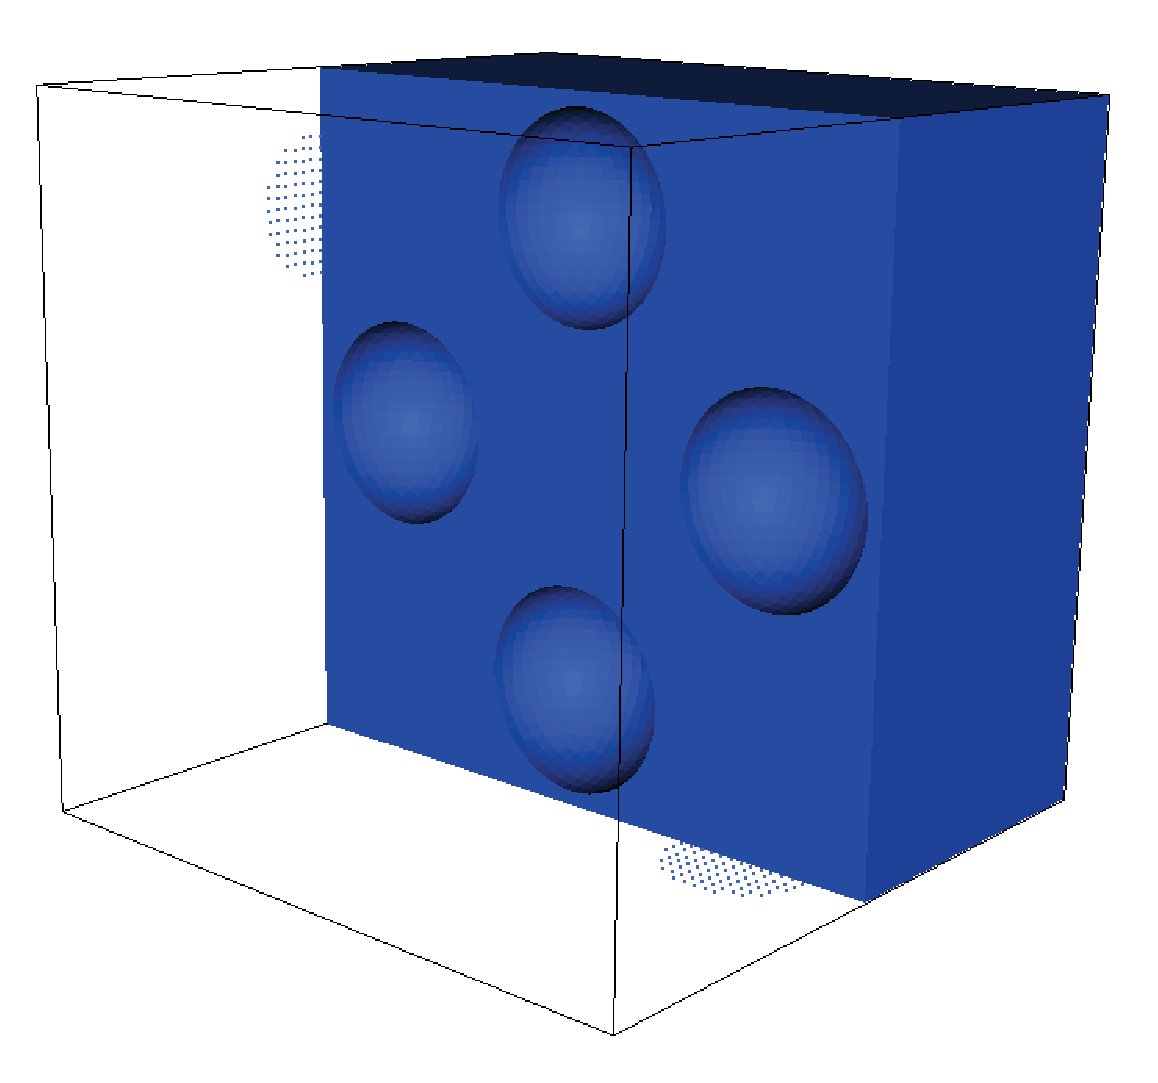
\includegraphics[width=\linewidth]{pipebend_initial_design_fluid.eps}
		} &
		\subfloat[Void phase.]{
			\label{fig:pipebend_initial_design_void}
			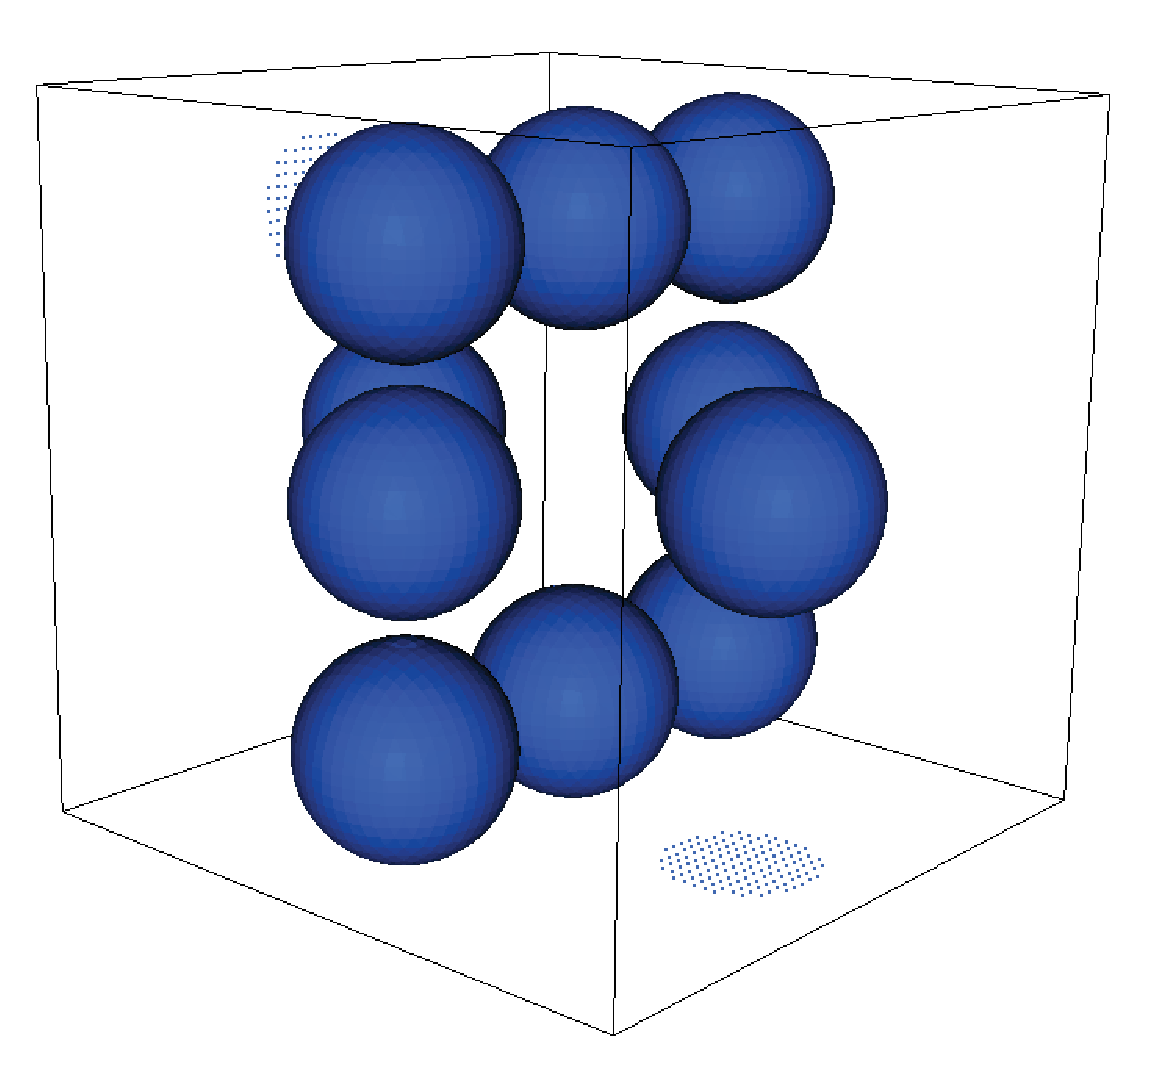
\includegraphics[width=\linewidth]{pipebend_initial_design_void.eps}
		}
	\end{tabularx}
	\caption{Initial designs for the pipe bend problem.}
	\label{fig:pipebend_initial_design}
\end{figure*}
%
\begin{figure*}
	\centering
	\begin{tabularx}{\linewidth}{XX}
		\subfloat[Symmetrical clip along the XY facet of the fluid phase.]{
			\label{fig:diffuser_initial_design_fluid}
			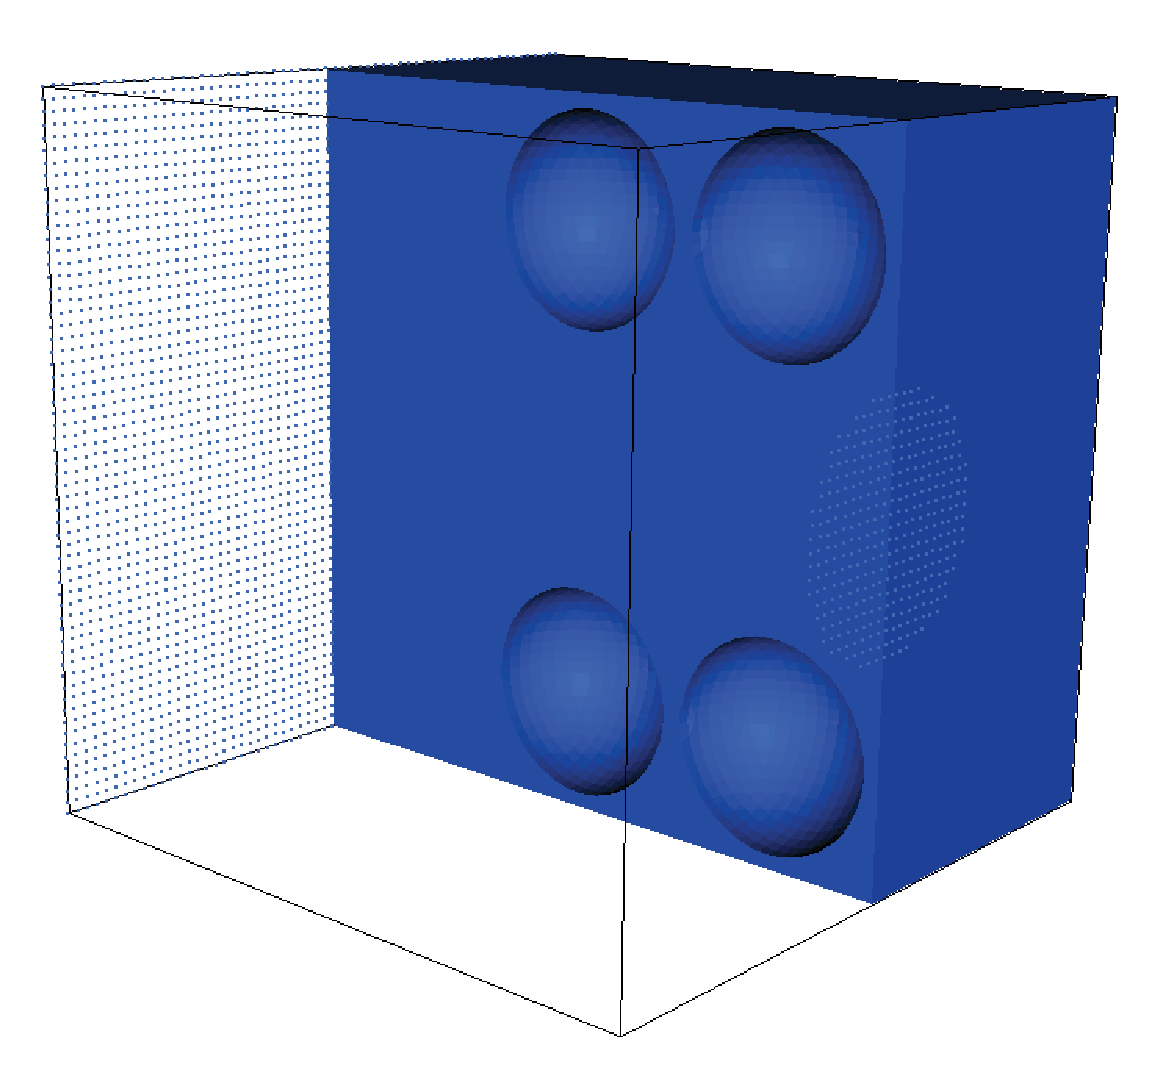
\includegraphics[width=\linewidth]{diffuser_initial_design_fluid.eps}
		} &
		\subfloat[Void phase.]{
			\label{fig:diffuser_initial_design_void}
			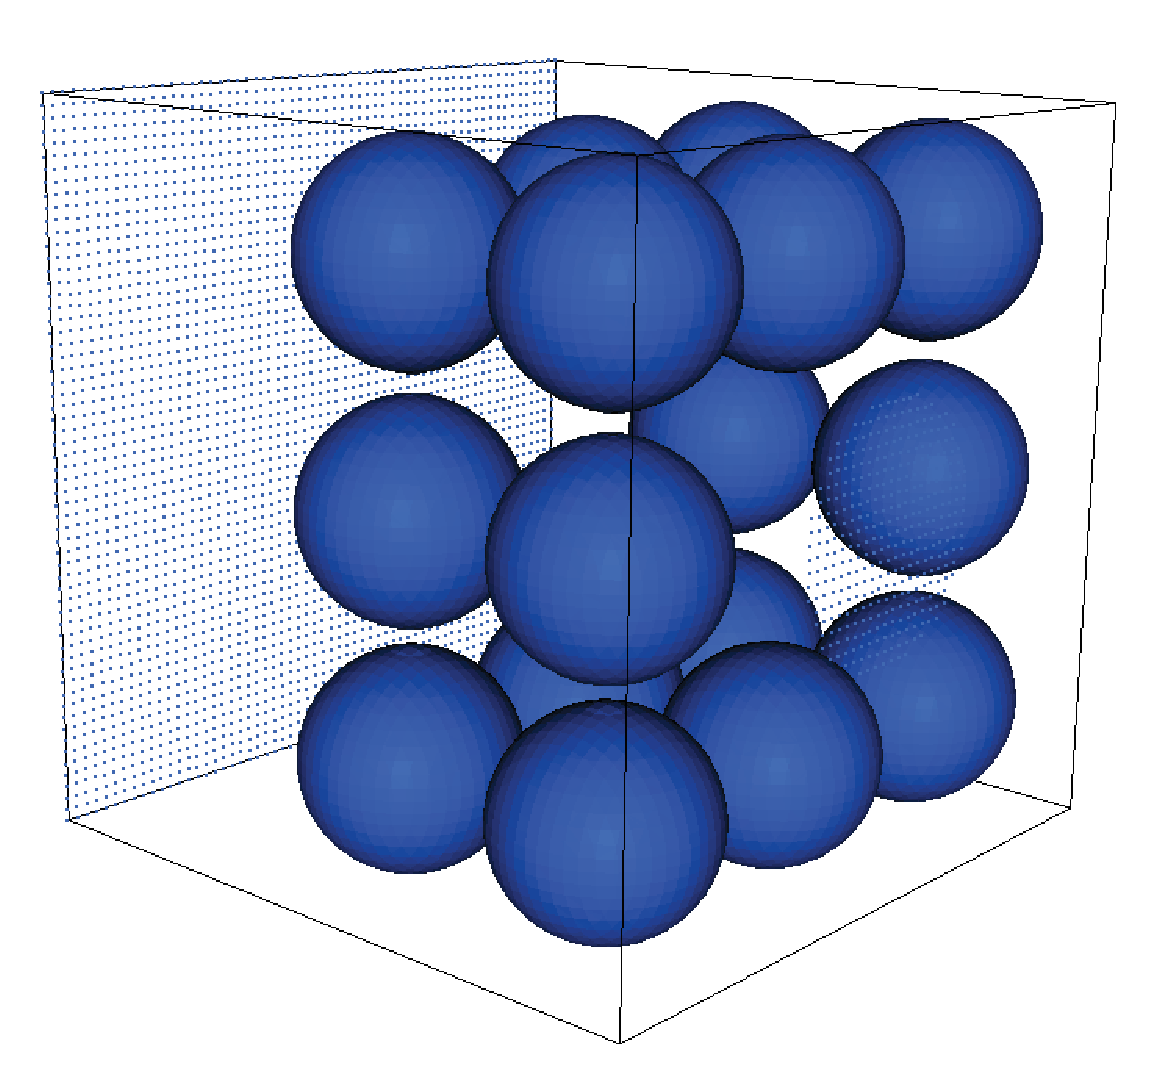
\includegraphics[width=\linewidth]{diffuser_initial_design_void.eps}
		}
	\end{tabularx}
	\caption{Initial designs for the diffuser problem.}
	\label{fig:diffuser_initial_design}
\end{figure*}
%
The objective for the bend and diffuser problems is defined as:
%
\begin{equation}
	\centering
	\label{eq:pipebend_diffuser_objective}
	\mathcal{F}_{\mathrm{bend/diffuser}} = w_{\mathrm{pres}} F_{\mathrm{PD}} + w_{\mathrm{per}} F_{\mathrm{perimeter}}
\end{equation}
%
\noindent
where $w_{\mathrm{pres}}$ and $w_{\mathrm{per}}$ are problem dependent parameters to penalize the pressure difference and perimeter objectives.

The volume fraction of the fluid phase is constrained as:
%
\begin{equation}
	\centering
	\label{eq:pipebend_diffuser_constraint}
	\mathcal{G}_{\mathrm{bend/diffuser}} = \frac{F_{\mathrm{volume},f}}{\bar{v}_{f} \left( F_{\mathrm{volume},f} + F_{\mathrm{volume},s} \right)} - 1
\end{equation}
%
\noindent
where $\bar{v}_{f}$ is the maximum volume fraction of the fluid phase.

Results for the Stokes and Navier-Stokes flows for a Reynolds number of $1$, for the bend and diffuser problems, yield the same optimized results and are shown in Figures \ref{fig:pipebend_results_stokes} and \ref{fig:diffuser_results_stokes}.
%
\begin{figure*}
	\centering
	\begin{tabularx}{\linewidth}{XX}
		\subfloat[Optimized geometry of the fluid phase.]{
			\label{fig:pipebend_results_stokes_fluid}
			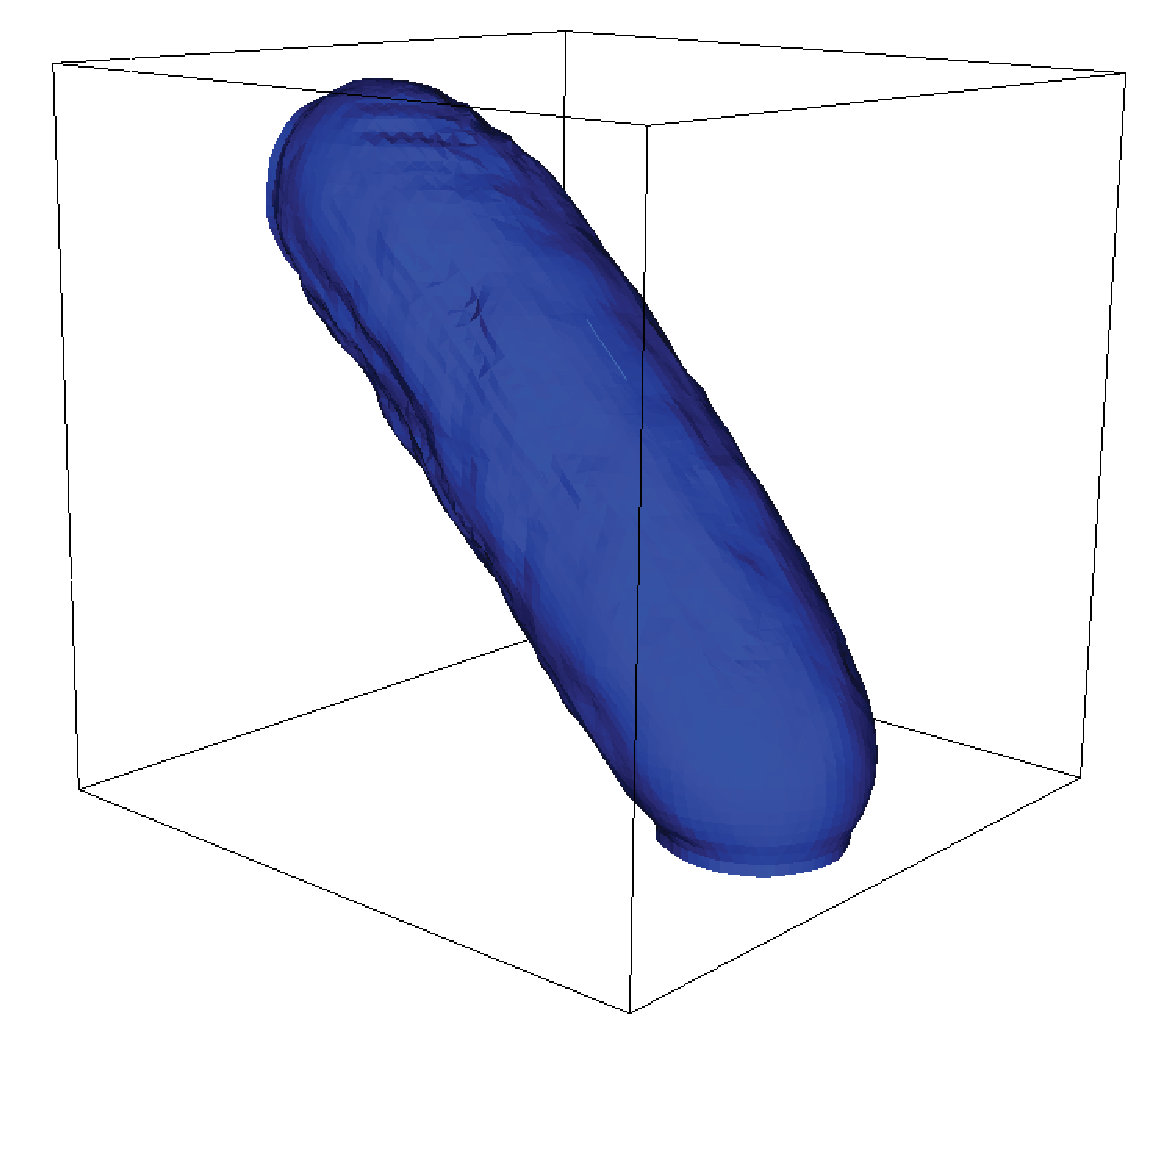
\includegraphics[width=\linewidth]{pipebend_results_stokes_fluid.eps}
		} &
		\subfloat[Symmetrical clip along the XY facet of the fluid phase. The black lines represent the streamlines of the flow. Legend shows magnitude of the velocity.]{
			\label{fig:pipebend_results_stokes_streamlines}
			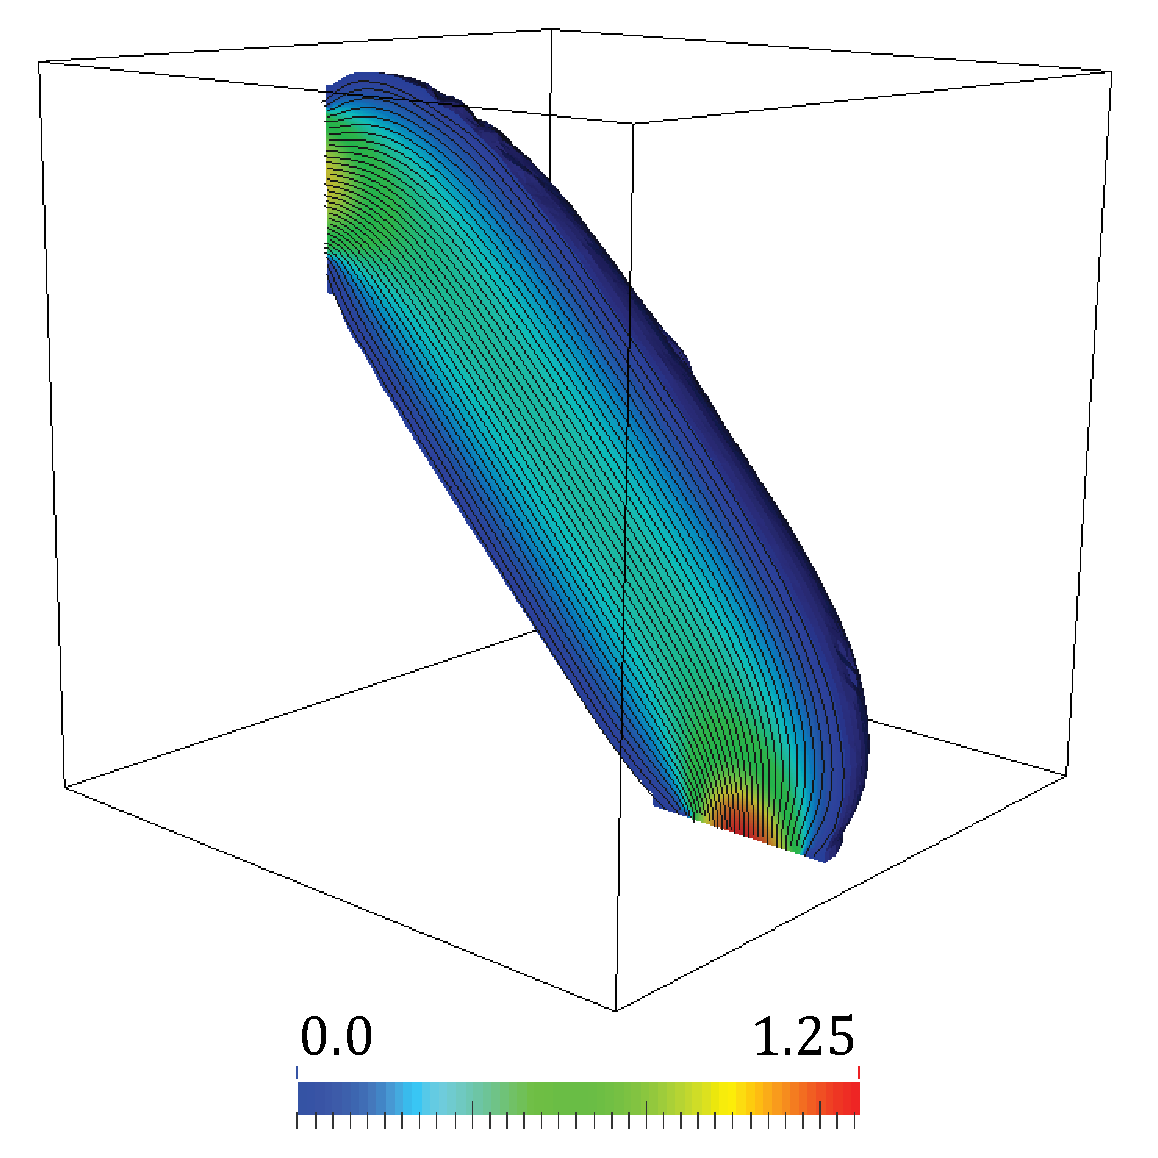
\includegraphics[width=\linewidth]{pipebend_results_stokes_streamlines.eps}
		}
	\end{tabularx}
	\caption{Results for the Stokes and Navier-Stokes pipebend optimization problems with a Reynolds number of $1$.}
	\label{fig:pipebend_results_stokes}
\end{figure*}
%
\begin{figure*}
	\centering
	\begin{tabularx}{\linewidth}{XX}
		\subfloat[Optimized geometry of the fluid phase.]{
			\label{fig:diffuser_results_stokes_fluid}
			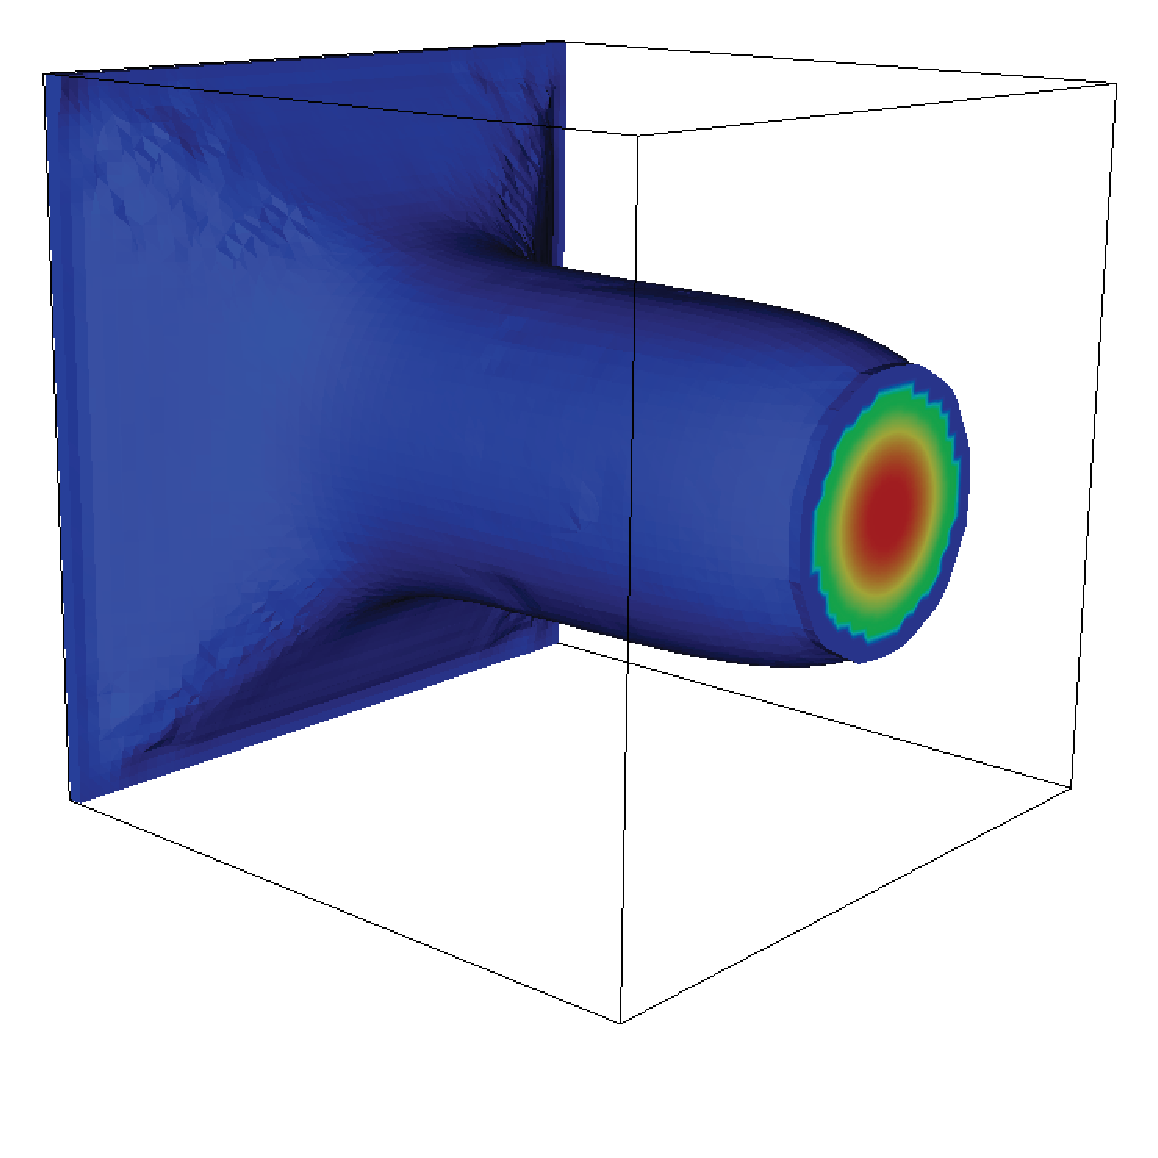
\includegraphics[width=\linewidth]{diffuser_results_stokes_fluid.eps}
		} &
		\subfloat[Symmetrical clip along the XY facet of the fluid phase. The black lines represent the streamlines of the flow. Legend shows magnitude of the velocity.]{
			\label{fig:diffuser_results_stokes_streamlines}
			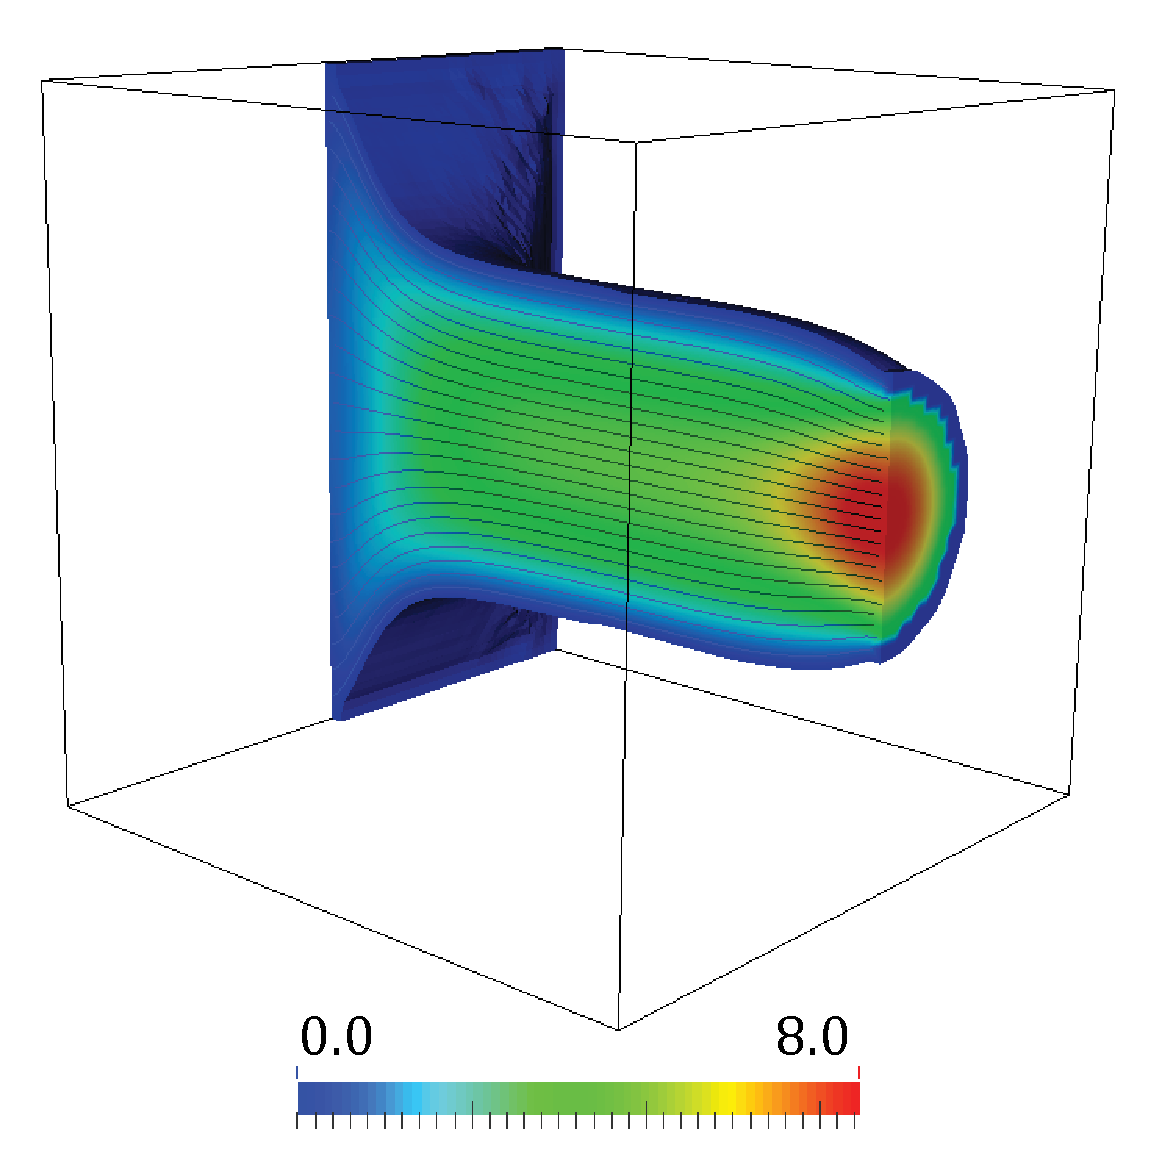
\includegraphics[width=\linewidth]{diffuser_results_stokes_streamlines.eps}
		}
	\end{tabularx}
	\caption{Results for the Stokes and Navier-Stokes diffuser optimization problems with a Reynolds number of $1$.}
	\label{fig:diffuser_results_stokes}
\end{figure*}
%
% -----------------------------------------------------------------------------

\subsection{Micromixer}
\label{sec:micromixer}
This example studies the optimization of a micromixer. This problem has been previously studied by using a homogenization method with a Brinkman penalization by \citep{MPY+:12} and by using a LSM-XFEM approach in two dimensions by \citep{MM:14}. The problem setup is defined in Figure \ref{fig:micromixer_setup}. A fluid with a scalar field value of $1.0$ and fluid with a value of $0.0$ enter the domain through a circular inclusion on the minimum YZ facet and leave through another circular inclusion on the maximum YZ facet. Both fluids are ideally miscible and have identical flow properties. The optimization problem consists in finding the optimal channel geometry that maximizes the mixing of the two fluids.
%
\begin{figure}
	\centering
	\includegraphics[width=0.75\linewidth]{micromixer_setup.eps}
	\caption{Setup for the micromixer problem. A parabolic inlet flow in the $x$-direction, with a maximum value of $1.0$ enters the design domain through a circular inclusion of diameter $L$ through the minimum YZ facet. The upper area of the inlet has a scalar value of $1.0$, while the lower area has a value of $0.0$. The outlet is located in the maximum YZ facet with a constant pressure of $1.0$.}
	\label{fig:micromixer_setup}
\end{figure}
%
The objective of the optimization problem is defined as
%
\begin{equation}
	\centering
	\label{eq:micromixer_objective}
	\mathcal{F}_{\mathrm{micromixer}} = F_{\mathrm{TSV}}
\end{equation}
%
with $\beta^{f} = 100$ and $T_{\mathrm{ref}}^{f} = 0.5$, which minimizes the maximum deviation of the scalar values of both fluids to the desired mixing value of $T_{\mathrm{ref}}^{f}$. Unlike the previous examples, a perimeter penalty is not used, as it would penalize the design towards a flat channel which would affect the maximization of the mixing.

Constraints are imposed on the maximum pressure drop to ensure the channel remains connected from the inlet to the outlet, and on the volume fraction of the fluid phase.
%
\begin{equation}
	\centering
	\label{eq:micromixer_constraint_1}
	\mathcal{G}_{\mathrm{micromixer,1}} = \frac{F_{\mathrm{PD}}}{\vartriangle p_{\mathrm{ref}}} - 1
\end{equation}
%
\begin{equation}
	\centering
	\label{eq:micromixer_constraint_2}
	\mathcal{G}_{\mathrm{micromixer,2}} = \frac{F_{\mathrm{volume},f}}{\bar{v}_{f}\left(F_{\mathrm{volume},f} + F_{\mathrm{volume},s} \right)} - 1
\end{equation}
%
The rest of the parameters for the problem are defined in Table \ref{tab:micromixer_parameters}.
%
\begin{table}
	\centering
	\begin{tabular*}{0.75\textwidth}{l l}
	\hline
	Outlet pressure             & 1.0 \\
	Reynolds number             & 1.0 \\
	Thermal conductivity        & $k^{f}_{xx} = 0.001$ \\
    Inlet velocity              & $u^{f}_{h_{x}} = 1.0$ \\
    Element length              & $h=0.166667$ \\
    Maximum volume fraction     & $\bar{v}_{f} = 0.5$ \\
	Maximum pressure drop       & $\vartriangle p_{\mathrm{ref}} = 1$ \\
	Smoothing filter            & $d = 2.4 \cdot h$ \\
	\hline
	\end{tabular*}
	\caption{Parameters for diffuser problem.}
	\label{tab:micromixer_parameters}
\end{table}
%
The optimized geometry for the Stokes and Navier-Stokes flows for a Reynolds number of $1$ yield the same optimized result, and is shown in Figure \ref{fig:micromixer_results_stokes_001}. The scalar field with a value of $T = 1.0$, the ``red'' fluid, and the field with a value of $T = 0.0$, the ``blue'' fluid, mix to create ``green'' fluid with a value of $T = 0.5$. The final design increases the length of the path traveled by the fluid, enhacing the mixing by creating multiple channels in all directions, similar to a ``twizzler''. 
%
\begin{figure*}
	\centering
	\begin{tabularx}{\linewidth}{XX}
		\subfloat[Optimized geometry of the fluid phase.]{
			\label{fig:micromixer_results_stokes_001_fluid}
			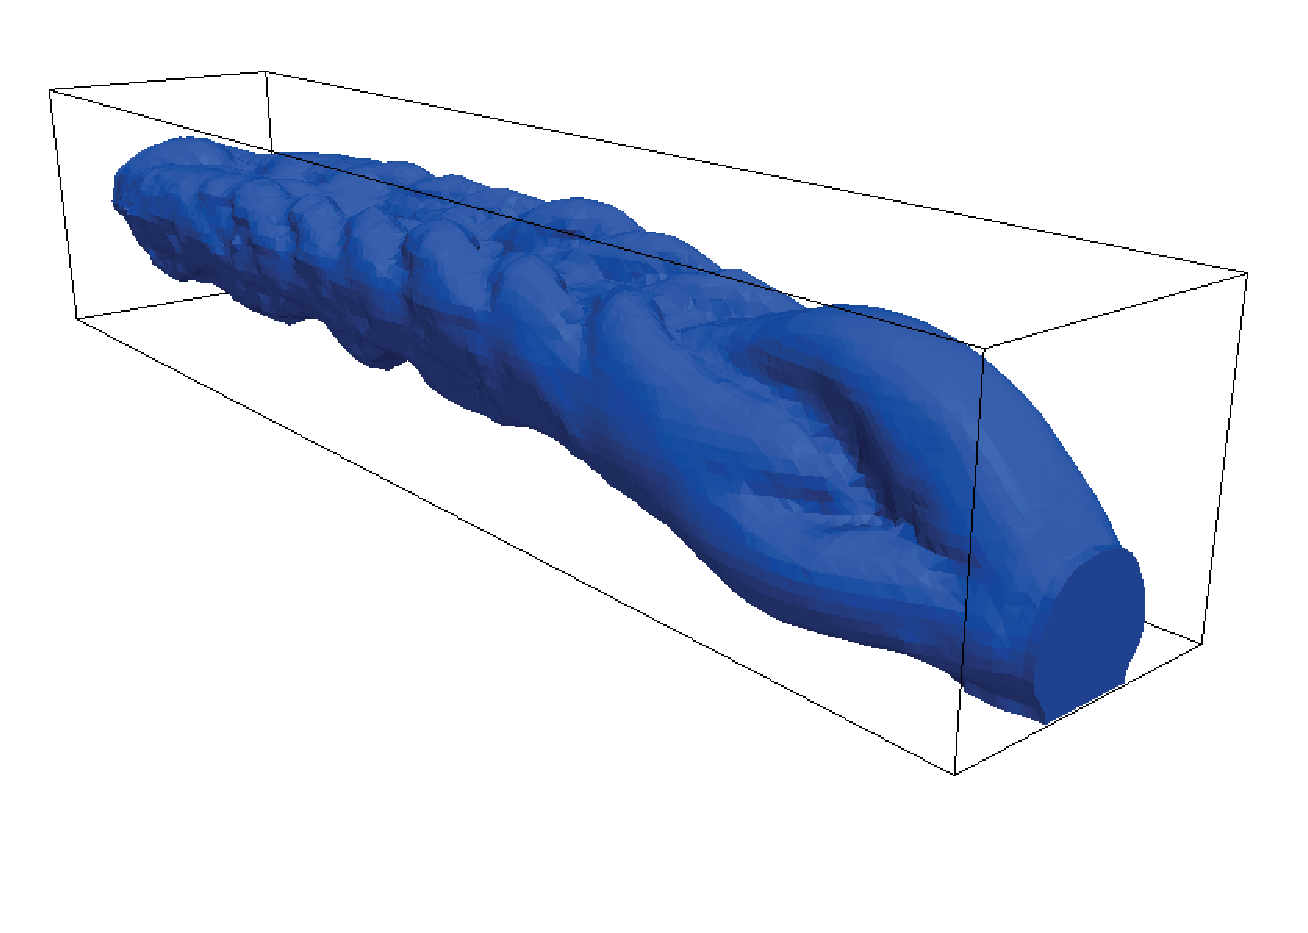
\includegraphics[width=\linewidth]{micromixer_results_stokes_001_fluid.eps}
		} &
		\subfloat[Scalar field distribution.]{
			\label{fig:micromixer_results_stokes_001_solution}
			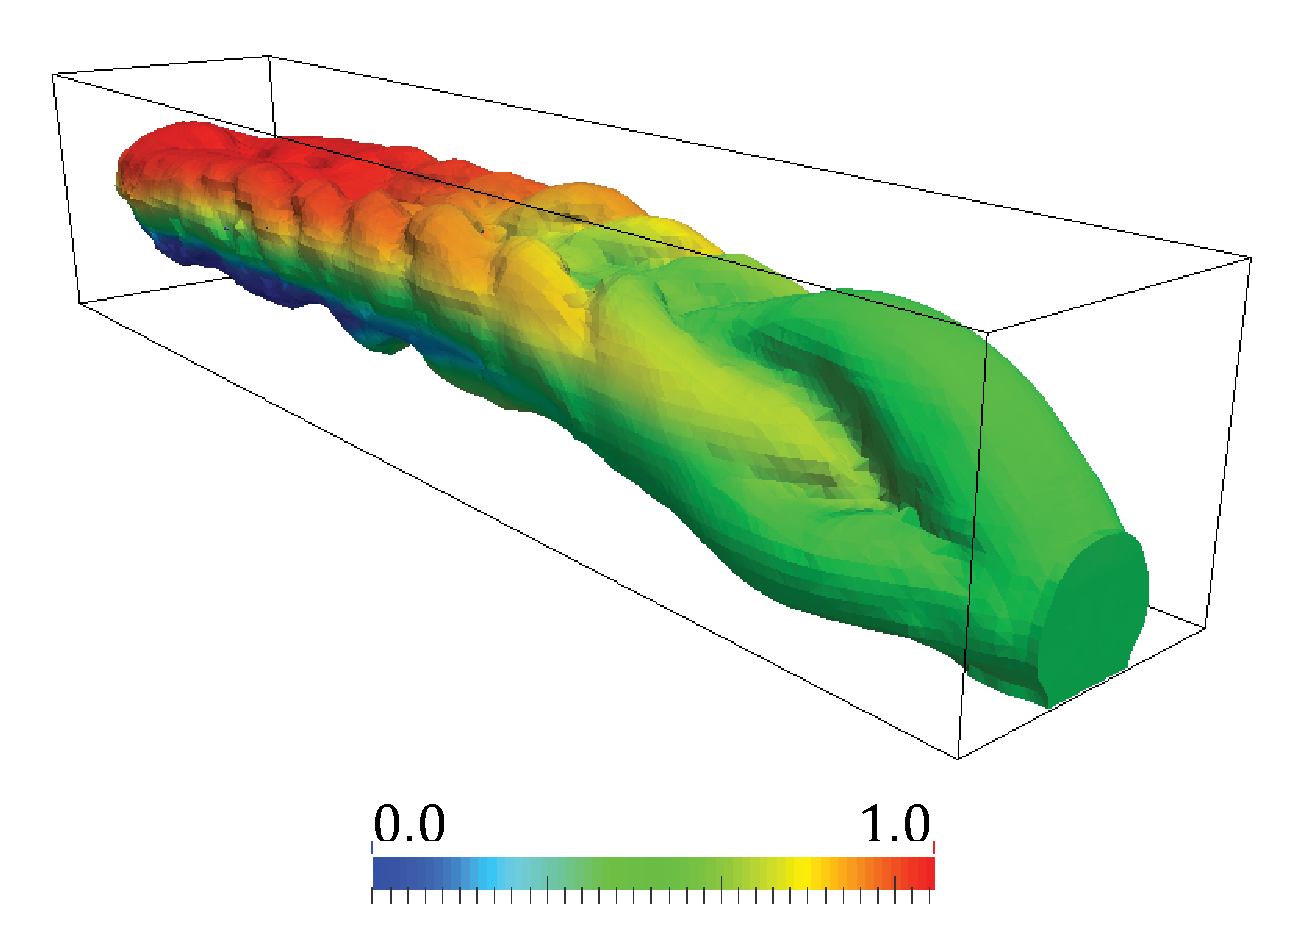
\includegraphics[width=\linewidth]{micromixer_results_stokes_001_solution.eps}
		} \\
		\subfloat[Top view of the optimized geometry.]{
			\label{fig:micromixer_results_stokes_001_top}
			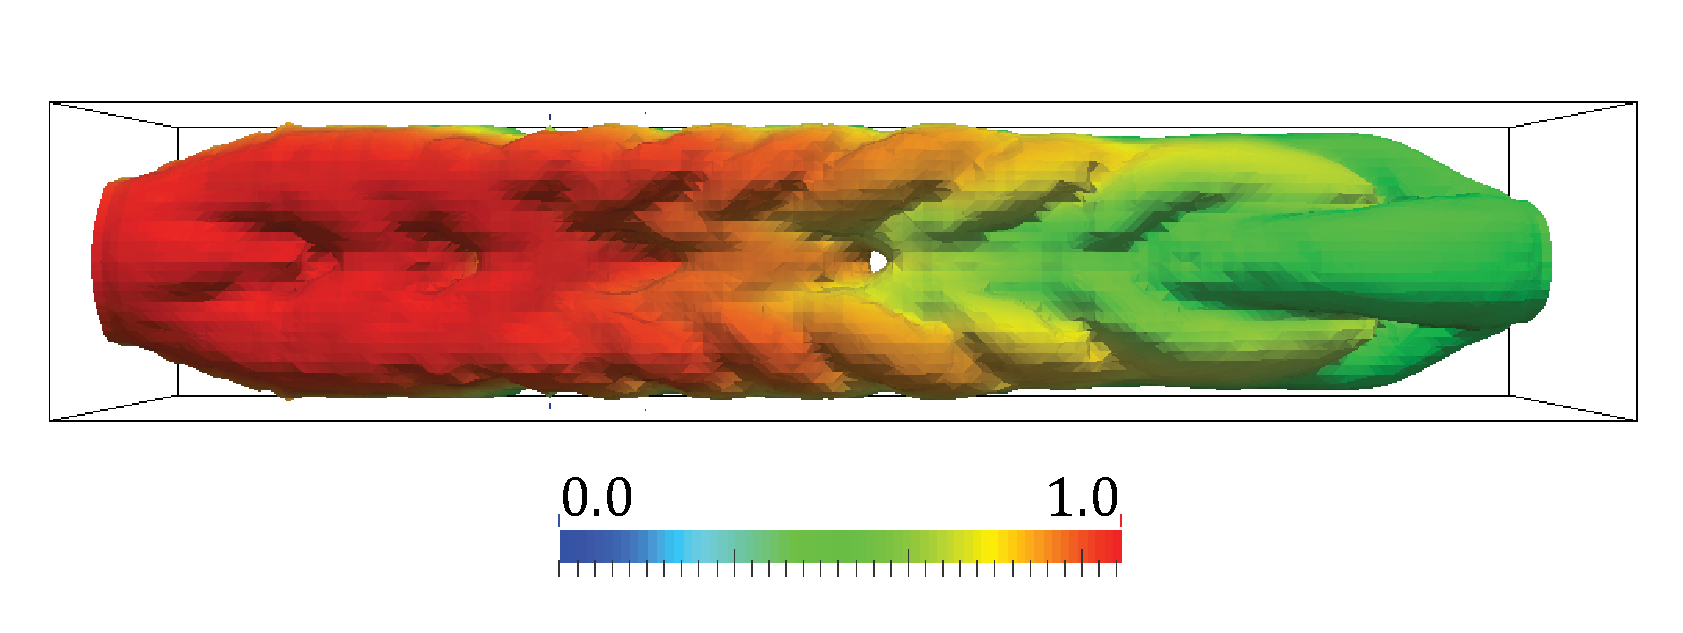
\includegraphics[width=\linewidth]{micromixer_results_stokes_001_top.eps}
		} &
		\subfloat[Bottom view of the optimized geometry.]{
			\label{fig:micromixer_results_stokes_001_bottom}
			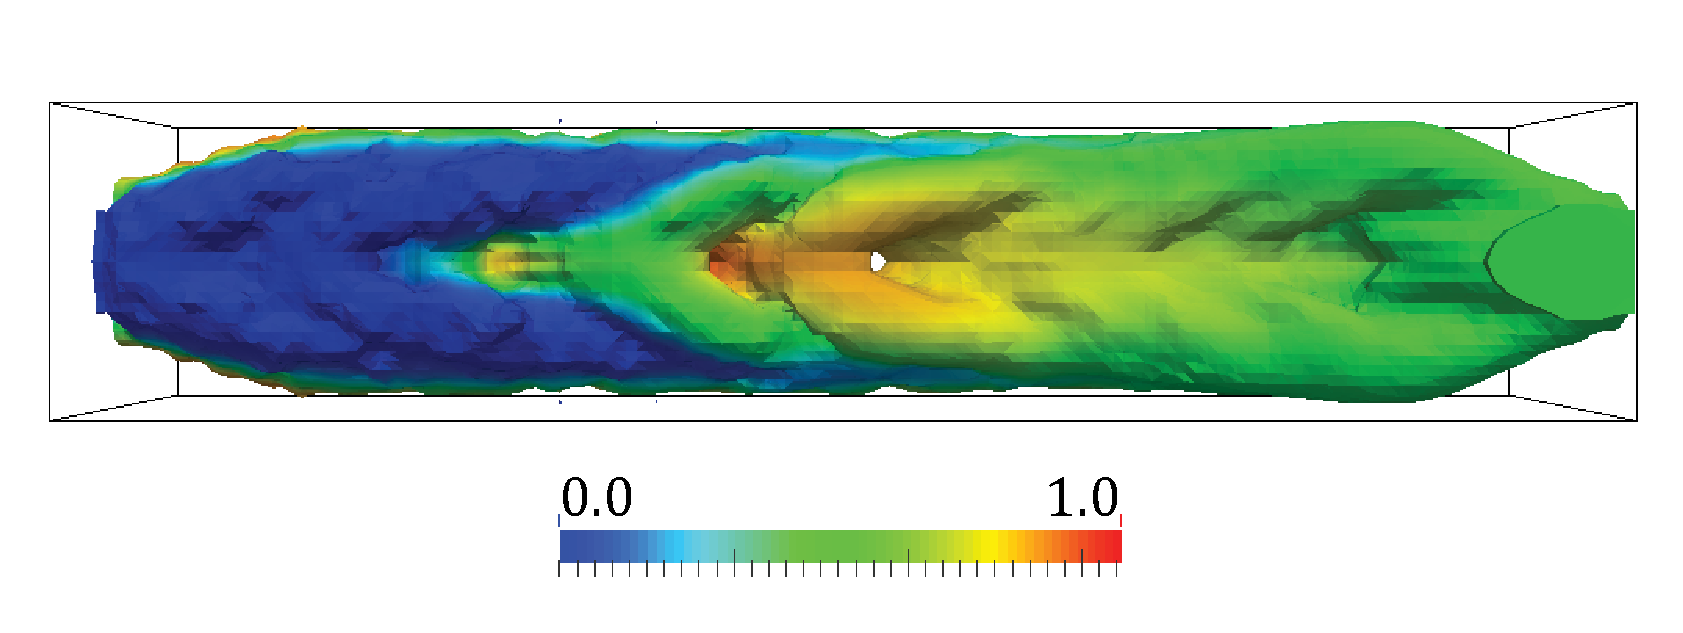
\includegraphics[width=\linewidth]{micromixer_results_stokes_001_bottom.eps}
		}
	\end{tabularx}
	\caption{Results for the Stokes and Navier-Stokes micromixer optimization problems with a Reynolds number of $1$ and a thermal conductivity of $k^{f}_{xx} = 0.001$. Legend shows the magnitude of the scalar field.}
	\label{fig:micromixer_results_stokes_001}
\end{figure*}

Streamlines of the fluid flow are shown in Figure \ref{fig:micromixer_streamlines_001}.
%
\begin{figure*}
	\centering
	\begin{tabularx}{\linewidth}{X}
		\subfloat[Streamlines along the XY facet.]{
			\label{fig:micromixer_streamlines_001_XY}
			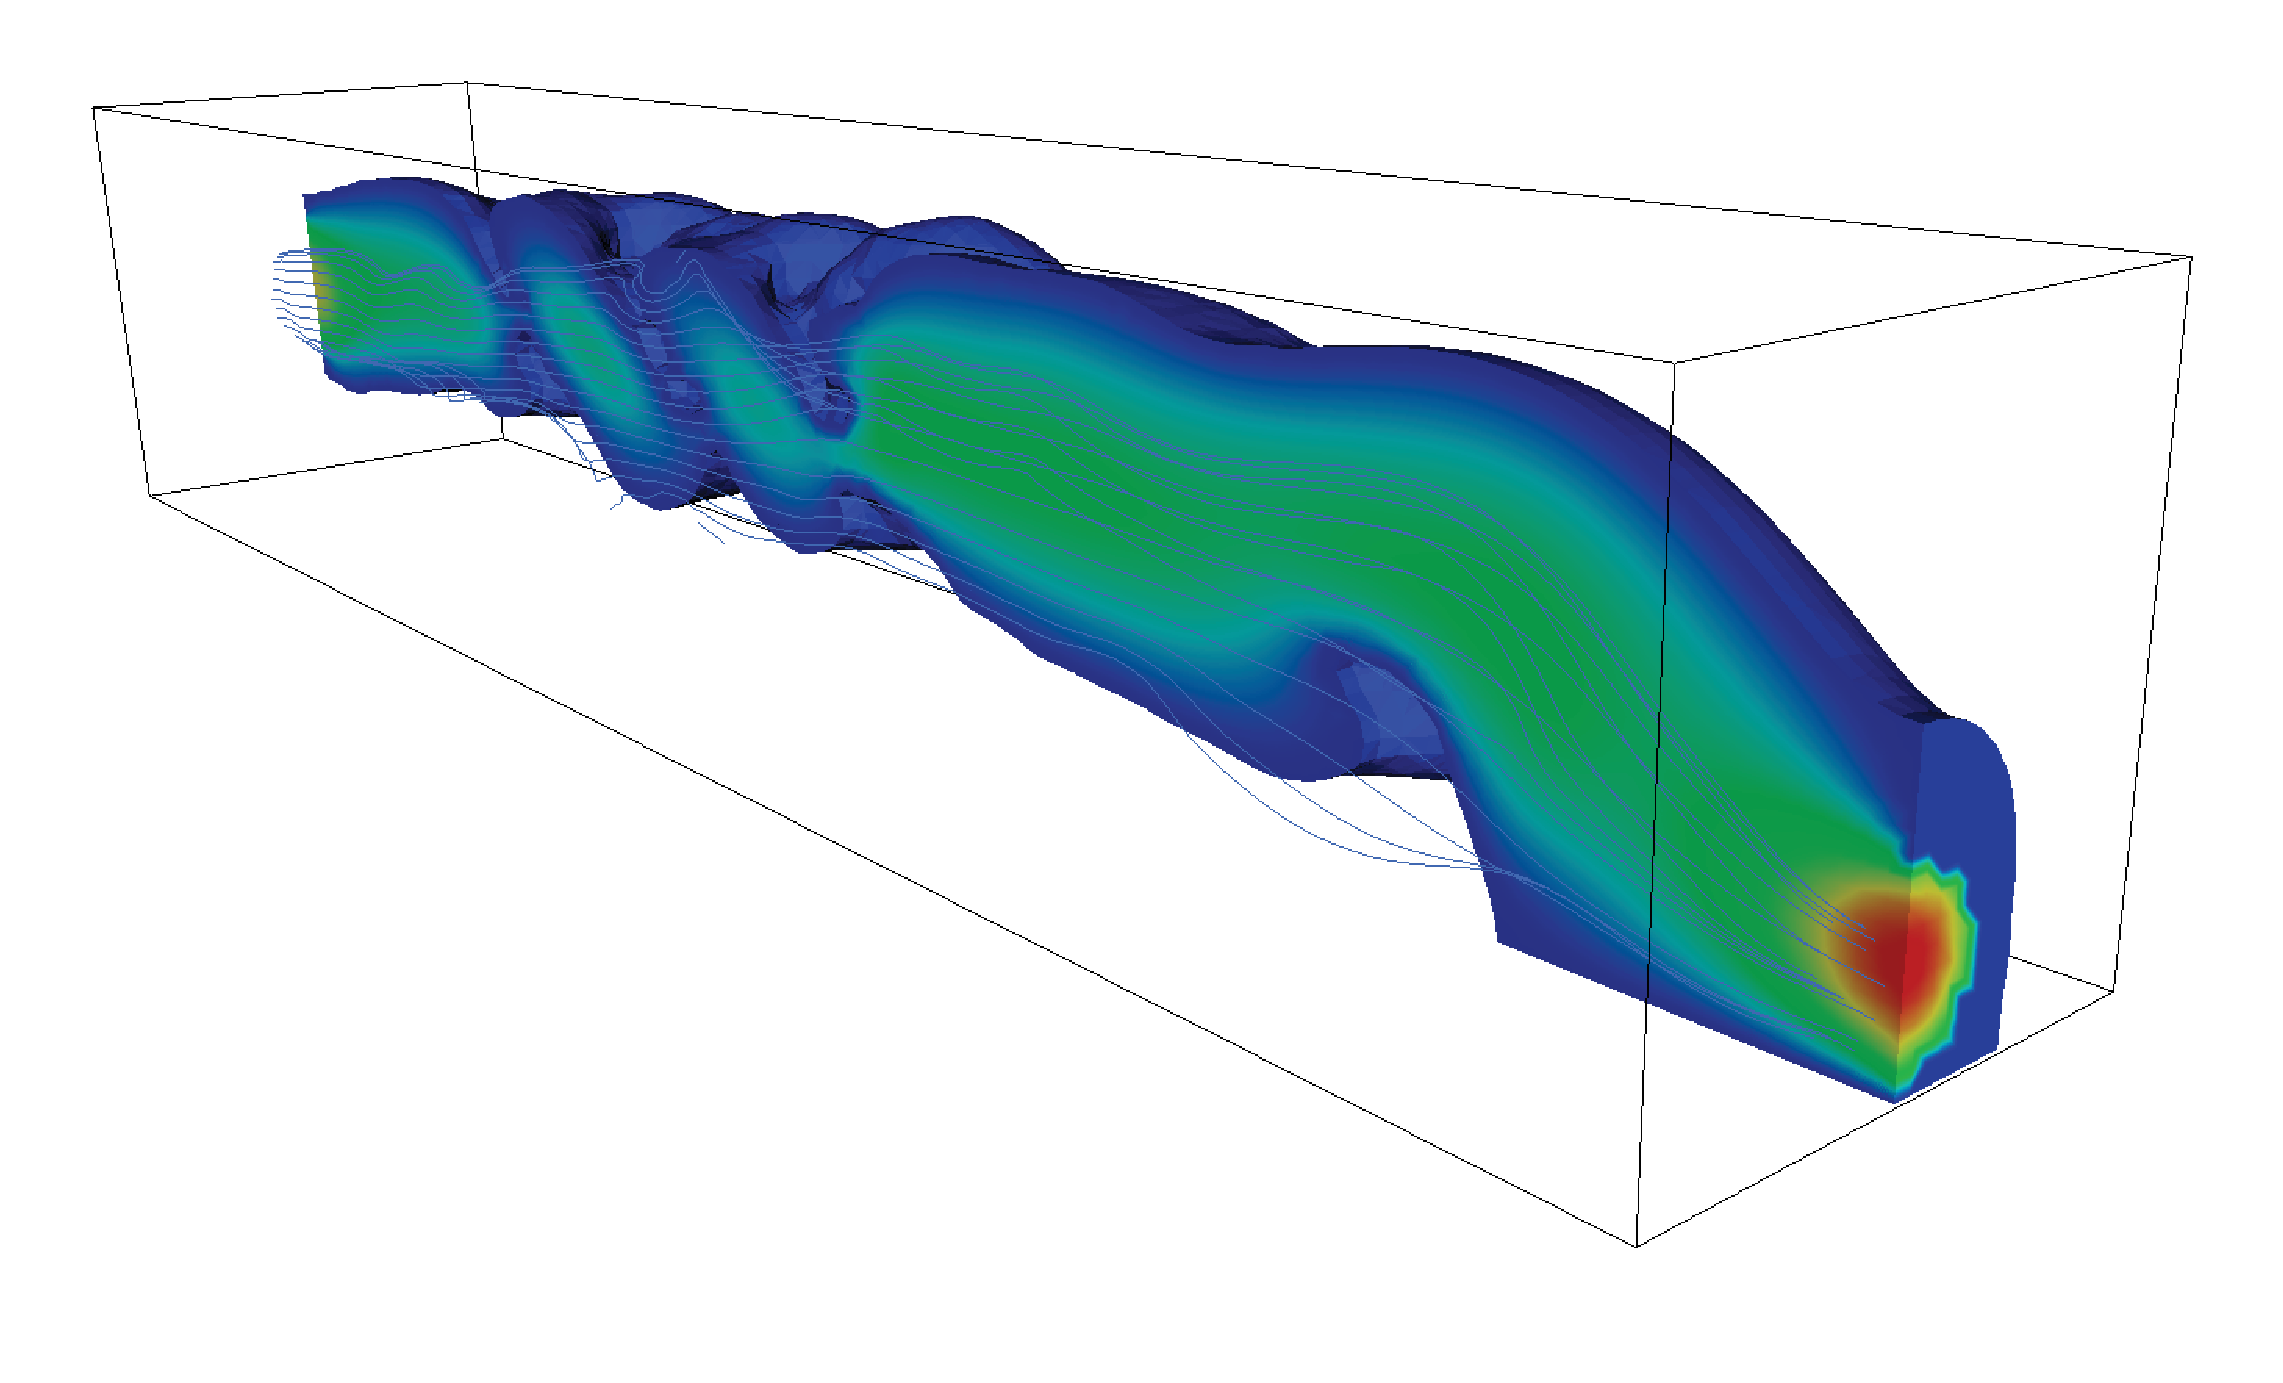
\includegraphics[width=\linewidth]{micromixer_streamlines_001_XY.eps}
		} \\
		\subfloat[Streamlines along the XZ facet.]{
			\label{fig:micromixer_streamlines_001_XZ}
			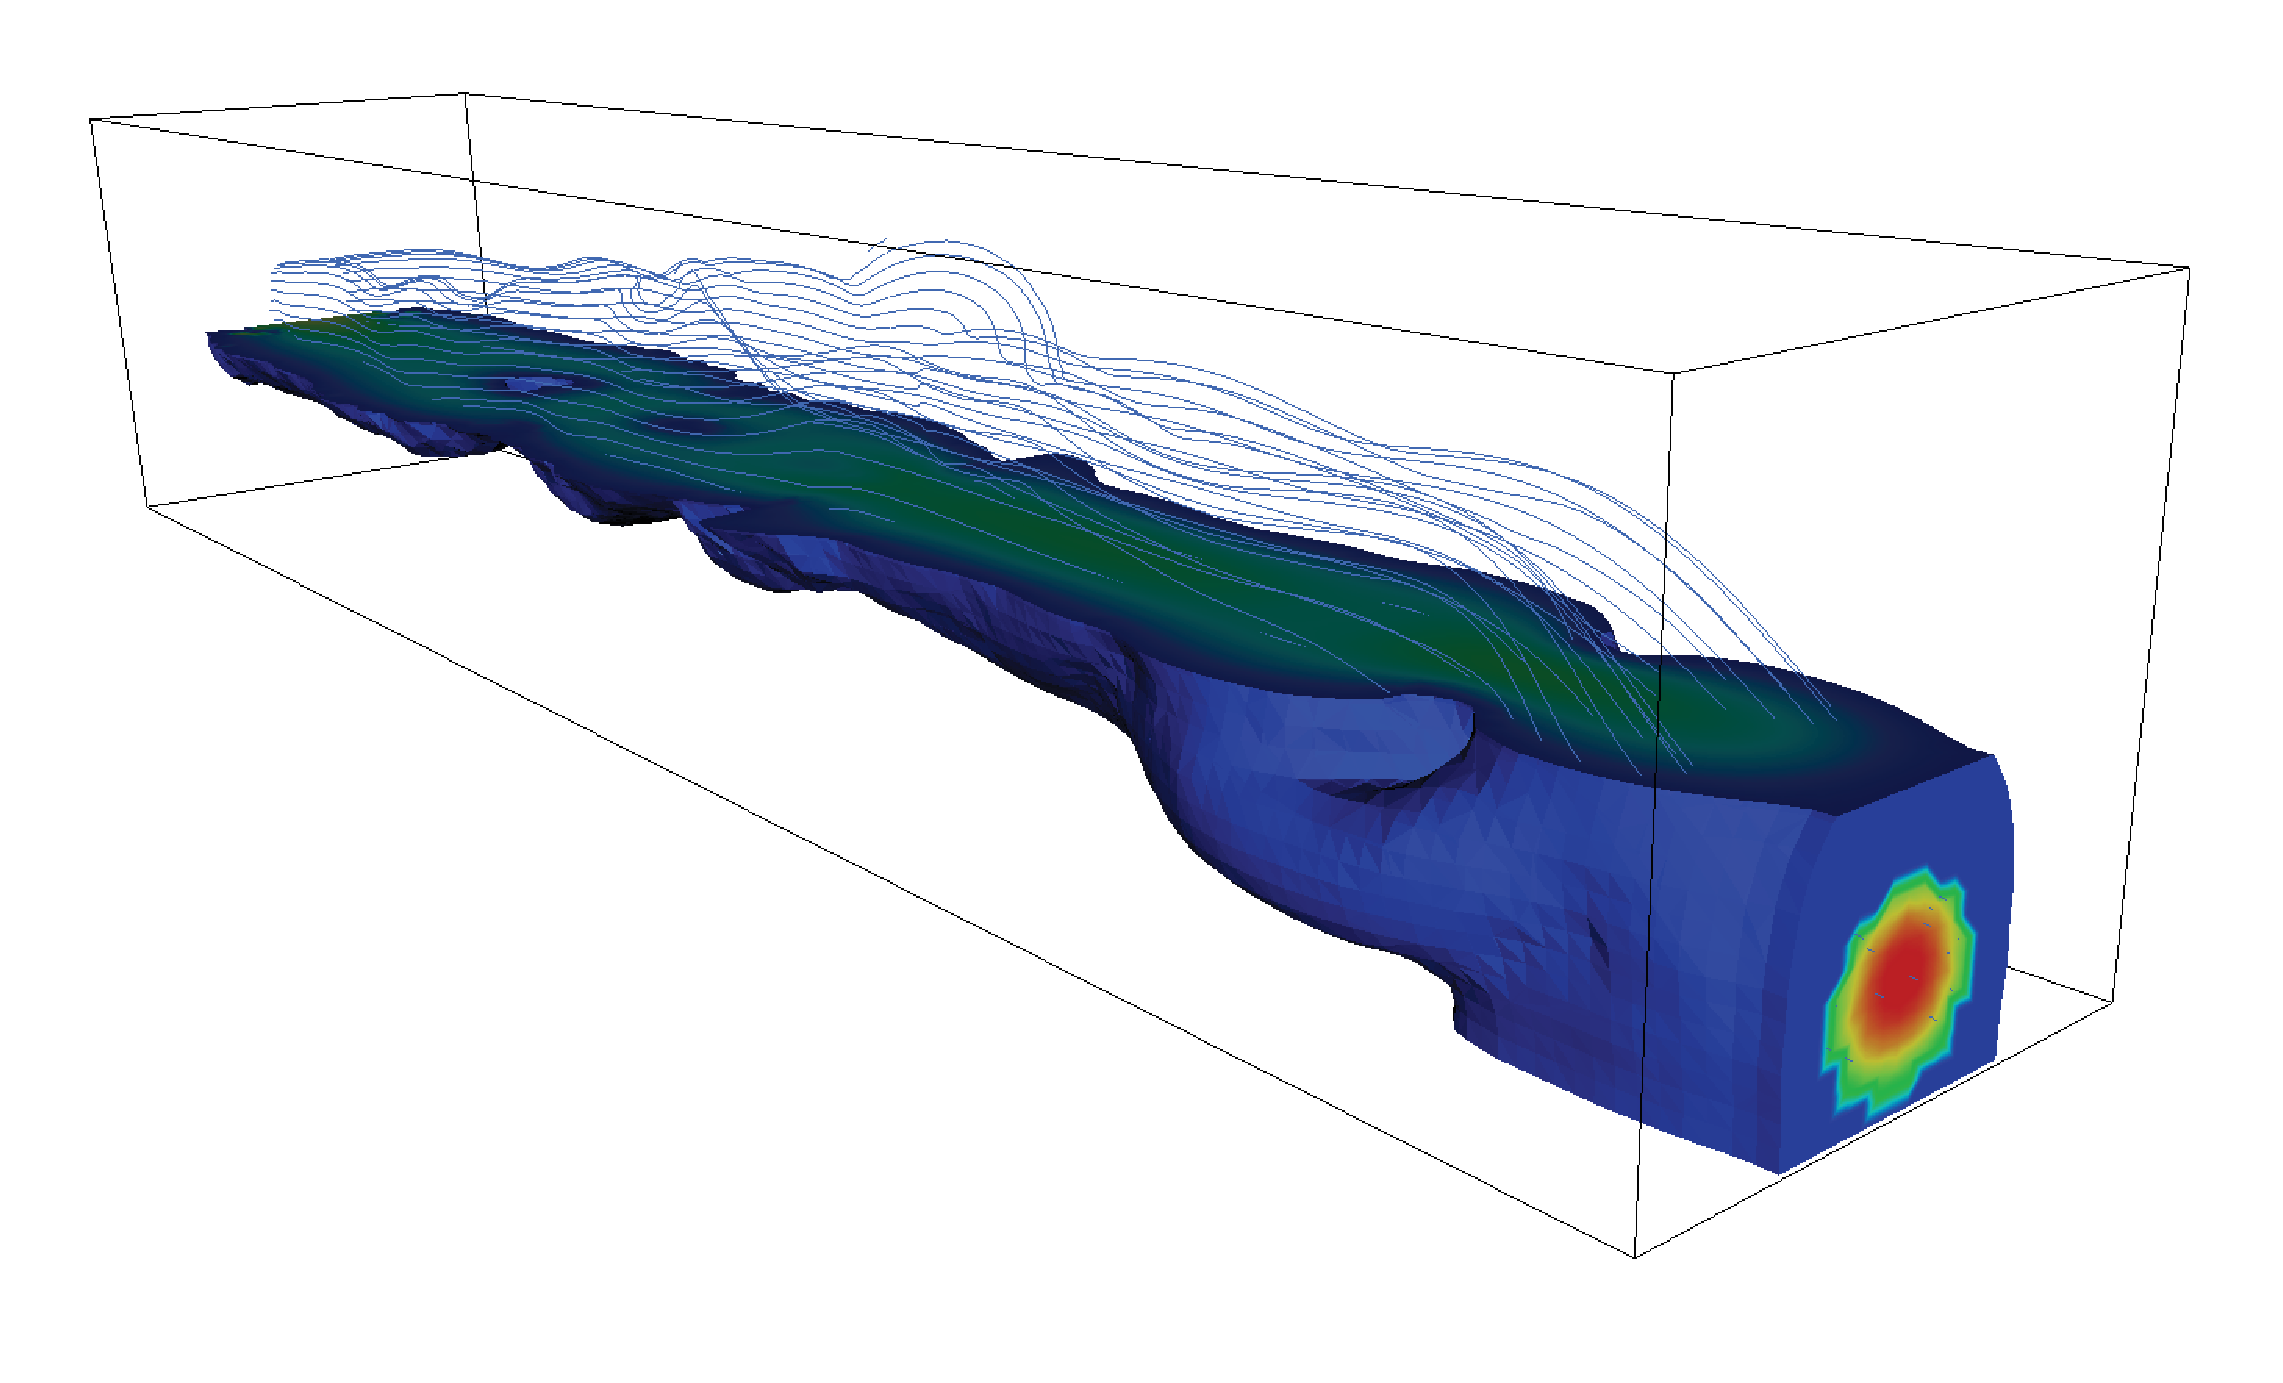
\includegraphics[width=\linewidth]{micromixer_streamlines_001_XZ.eps}
		}
	\end{tabularx}
	\caption{Streamlines for the Stokes and Navier-Stokes micromixer optimization problems with a Reynolds number of $1$ and a thermal conductivity of $k^{f}_{xx} = 0.001$.}
	\label{fig:micromixer_streamlines_001}
\end{figure*}
%
% -----------------------------------------------------------------------------

\section{Conclusions}
\label{sec:fluids_conclusions}

The LSM-XFEM framework was extended to three-dimensional incompressible Navier-Stokes flows and scalar transport optimization problems. Preliminary results show that high Reynolds number flows cannot be modeled accurately without the ghost penalty formulation.

To conclude this work, the author will implement the face-oriented ghost-penalty to formulate a robust optimization framework and be able to solve high Reynolds number flows. Curvature minimization approaches will be studied to generate smooth surfaces that facilitate the manufacturing of the optimized geometries via three dimensional printing.

% -----------------------------------------------------------------------------
% Acknowledgement

% \subsection*{Acknowledgement}
% 
% The authors acknowledge the support of the National Science Foundation under grant EFRI-ODISSEI  1240374 and CBET 1246854. The opinions and conclusions presented in this paper are those of the authors and do not necessarily reflect the views of the sponsoring organization.

% -----------------------------------------------------------------------------
% Bibliography

% \bibliographystyle{etc/spbasic}
% \bibliography{etc/JabRefDatabase}

% \end{document}
